\documentclass{article}

\usepackage{graphicx} %package to manage images
\graphicspath{ {./images/} }

\usepackage[rightcaption]{sidecap}

\usepackage{wrapfig}

\begin{document}

%----------------------------------------------------------------------------
%Here begins the simplest example. Importing an image with no extra parameters
The universe is immense and it seems to be homogeneous, in a large scale, everywhere we look at.

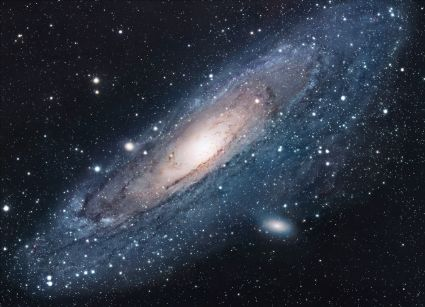
\includegraphics{universe}

There's a picture of a galaxy above
%----------------------------------------------------------------------------

\vspace{1.5cm}

%----------------------------------------------------------------------------
%Second example, scaling and image
Overleaf is a great professional tool to edit online documents, 
share and backup your \LaTeX projects. Also offers a 
rather large help documentation.


\includegraphics[scale=1.5]{overleaf-logo}
%----------------------------------------------------------------------------

\newpage

%----------------------------------------------------------------------------
%Third example, setting specific width and height
Overleaf is a great professional tool to edit online documents, 
share and backup your \LaTeX projects. Also offers a 
rather large help documentation.


\includegraphics[width=5cm, height=4cm]{overleaf-logo}
%----------------------------------------------------------------------------

\vspace{1.5cm}

%----------------------------------------------------------------------------
%Importing Images example, rotating
Overleaf is a great professional tool to edit online, 
share and backup your \LaTeX projects. Also offers a 
rather large base of help documentation.


\includegraphics[scale=1.2, angle=45]{overleaf-logo}
%----------------------------------------------------------------------------

\newpage

%----------------------------------------------------------------------------
%Importing Images example, alternative units
The universe is immense and it seems to be homogeneous, in a large scale, everywhere we look at.

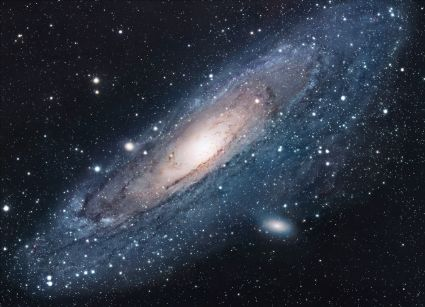
\includegraphics[width=\textwidth]{universe}
%----------------------------------------------------------------------------

\vspace{1.5cm}

%----------------------------------------------------------------------------
%Example, placing images
In the next example the figure will be positioned right below this sentence.

\begin{figure}[h]
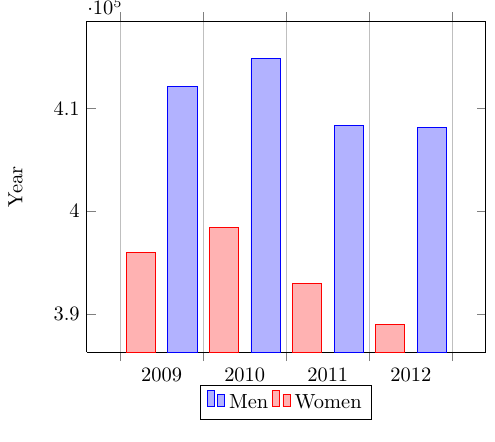
\includegraphics[width=8cm]{Plot}
\end{figure}
%----------------------------------------------------------------------------

\newpage

%----------------------------------------------------------------------------
%Example the image will be at the top
In this picture you can see a bar graph that shows
the results of a survey which involved some tricky
data studied as time passed.

\begin{figure}[t]
\centering
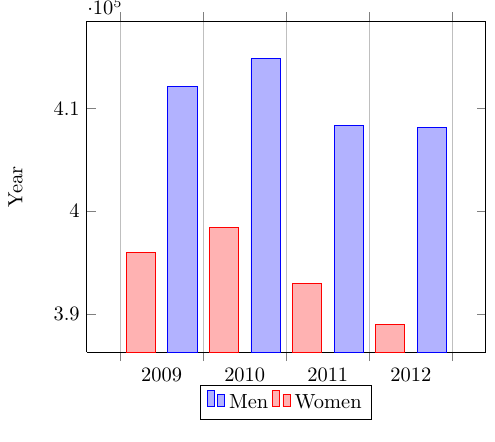
\includegraphics[width=8cm]{Plot}
\end{figure}
%----------------------------------------------------------------------------

\newpage

%----------------------------------------------------------------------------
%Example, floating pictures. Text wrapping the figure

\begin{wrapfigure}{r}{0.25\textwidth} %this figure will be at the right
    \centering
    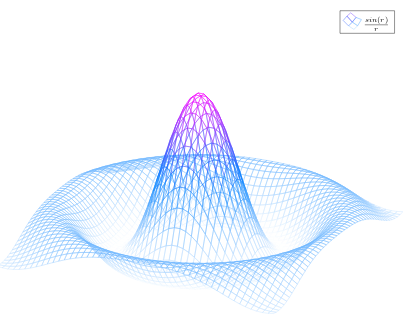
\includegraphics[width=0.25\textwidth]{mesh}
\end{wrapfigure}

\vspace{1.2cm}

There are several ways to plot a function of two variables, depending on the information you are interested in. For instance, if you want to see the mesh of a function so it easier to see the derivative you can use a plot like the one on the left.


\begin{wrapfigure}{l}{0.25\textwidth} %this figure will be at the left
    \centering
    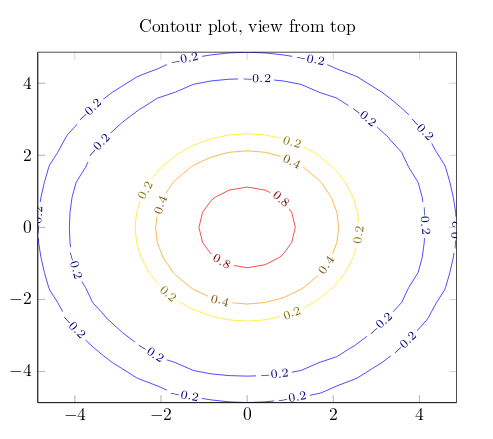
\includegraphics[width=0.25\textwidth]{contour}
\end{wrapfigure}

On the other side, if you are only interested on certain values you can use the contour plot, you can use the contour plot, you can use the contour plot, you can use the contour plot, you can use the contour plot, you can use the contour plot, you can use the contour plot, like the one on the left.

On the other side, if you are only interested on certain values you can use the contour plot, you can use the contour plot, you can use the contour plot, you can use the contour plot, you can use the contour plot, you can use the contour plot, you can use the contour plot, like the one on the left.

On the other side, if you are only interested on certain values you can use the contour plot, you can use the contour plot, you can use the contour plot, you can use the contour plot, you can use the contour plot, you can use the contour plot, you can use the contour plot, like the one on the left.
%----------------------------------------------------------------------------

\newpage

%----------------------------------------------------------------------------
%Example of captioning
\begin{figure}[h]
\caption{Example of a parametric plot ($\sin (x), \cos(x), x$)}
\centering
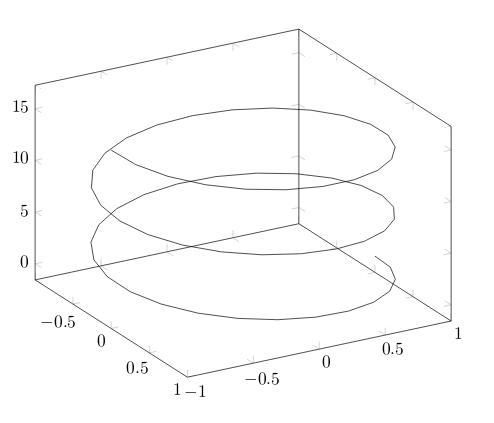
\includegraphics[width=0.6\textwidth]{spiral}
\end{figure}
%----------------------------------------------------------------------------

\vspace{1.5cm}

%----------------------------------------------------------------------------
%Example of caption next to the figure
\begin{SCfigure}[0.5][h]
\caption{Using again the picture of the universe. 
         This caption will be on the right}
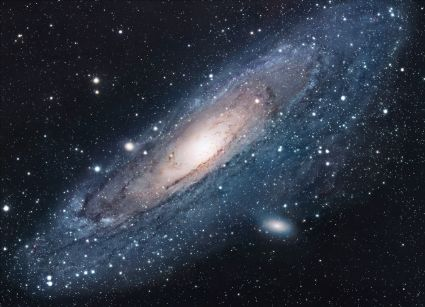
\includegraphics[width=0.6\textwidth]{universe}
\end{SCfigure}
%----------------------------------------------------------------------------


\newpage

%----------------------------------------------------------------------------
%Labeling and referencing example
\begin{figure}[h]
    \centering
    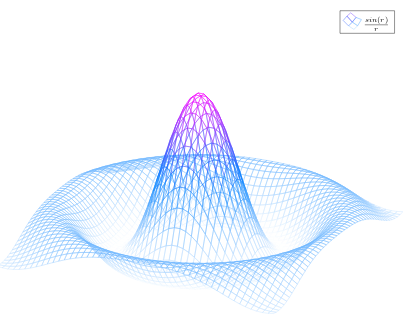
\includegraphics[width=0.25\textwidth]{mesh}
    \caption{a nice plot}
    \label{fig:mesh1}
\end{figure}

As you can see in the figure \ref{fig:mesh1}, the function grows near 0. Also, in the page \pageref{fig:mesh1} is the same example.
%----------------------------------------------------------------------------


%----------------------------------------------------------------------------
%This is a dummy example to generate the images index.
\begin{figure}[h]
    \centering
    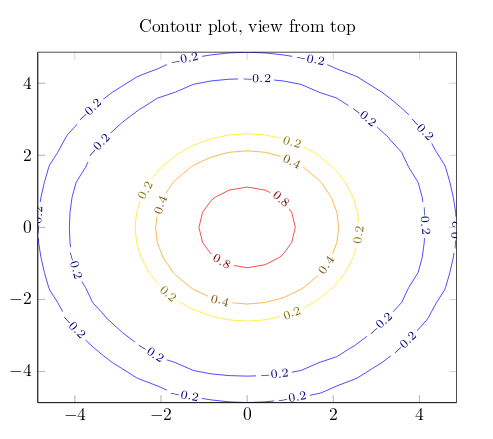
\includegraphics[width=0.25\textwidth]{contour}
    \caption{a nice contour plot}
    \label{fig:mesh2}
\end{figure}
%----------------------------------------------------------------------------

\newpage

%----------------------------------------------------------------------------
%Generating a list of figures

\listoffigures

%----------------------------------------------------------------------------

\end{document}


